\documentclass[11pt]{article}
\usepackage[cache=false]{minted}

\usepackage[utf8]{inputenc} 
\usepackage[T1]{fontenc}
\usepackage{lmodern}
\usepackage[ngerman]{babel}
\usepackage{hyperref}
\usepackage{graphicx}
\usepackage{float}
\usepackage{tabularx}
\usepackage{caption}
\usepackage{copyrightbox}

\graphicspath{{pictures/}}

\title{Ein Einführung in GraphQL}
\author{Jannik Wojnar}
\date{\today}

\begin{document}


\maketitle
\paragraph{}
Dieses Dokument soll eine generelle Einführung in das Thema Graphql geben. Vorausgesetzt werden grundlegende Kenntnisse der Service Orientierten Architektur (SOA). Abschließend wird auf den Nutzen von GraphQL in der Wirtschaft eingegangen und ein Ausblick auf die Zukunft gegeben.

\tableofcontents
\newpage

\section{Einführung in GraphQL}
GrahpQL ist eine Datenabfrage und Manipulationssprache, welche 2012 von Facebook entwickelt wurde und 2015 erschienen ist. 2018 wurde  das Projekt der Linux Foundation übertragen.
Im Allgemeinen kann zunächst festgestellt werden dass in GraphQL die Informationen die vom Server an den Clienten ausgeliefert werden sollen genauer vom Clienten festgelegt werden können (als beispielsweise bei einer herkömmlichen REST Schnittstelle). Dies wird als einer der größten Vorteile von GraphQL betrachtet.
Im Folgenden soll GraphQL im Kontext einer klassische Client-Server-Architektur vorgestellt werden.

\subsection{Server}
Im Unterschied zu etablierten Schnittstellen Architekturen werden bei GraphQL Daten lediglich über nur einen Endpunkt angefragt. An diesen werden im Normalfall mittels HTTP-Verb POST Anfragen an den Server gestellt.

\subsubsection{Schema}
Wie diese Anfragen aussehen dürfen und welche Daten damit abgefragt werden können wird durch ein sogenanntes \textit{Schema} festgelegt, in welchem Daten und Anfragen stark typisiert definiert sind.
Das \textit{Schema} kann als ein Graph verstanden werden der die Gesamtmenge aller möglichen Anfragen an die Schnittstelle darstellt. Es wird mittels der \textit{Schema Definition Language} (SDL) beschrieben und stellt eine festen Bezugspunkt dar der die Schnittstelle klar definiert. Die dadurch generierte hohe Sichtbarkeit kann zu einer unabhängigen Entwicklung von Frontend und Backend genutzt werden.
 Zur Verdeutlichung der Funktionsweise eines Schema soll im Folgenden ein Beispiel Schema definiert werden und an diesem auch weitere Funktionalitäten erläutert werden.
 
\paragraph{Scalars und Datentypen}
Basierend auf den \textit{Scalar} Typen String, Int, Float, Boolean und ID können \textit{Datentypen} definiert werden. Diese können auch Relationen untereinander aufweisen. An den tiefsten/untersten Punkten eines Schema stehen also immer skalare Typen, die bildhaft betrachtet die Blätter des Schemas darstellen.

\begin{minted}{javascript}
	type Book {
	 	id: String!
		title: String
		published: Boolean!
	}

	type Author {
		name: String!
		books: [Book!]!
	}
\end{minted}

\paragraph{Schnittstellen}
Für die Definition der obersten Punkte eines Schemas, welche die Einstiegspunkte für Anfragen darstellen, werden die drei \textit{root} Typen  \textit{Query, Mutation} und  \textit{Subscription} verwendet. Diese stellen die Anfangspunkte einer möglichen Anfrage dar. Um nun genauer zu definieren welche Daten und in welcher Form diese zurückgegeben werden, werden die zuvor definierten Datentypen genutzt. 

\begin{minted}{javascript}
	type Query {
		allAuthors: [Author!]
		allBooks: [Book!]
		authorById(id: int!): Author
	}

	type Mutations {
		createNewAuthor(name: String!, books: [books!]!): Author!
		createNewBook(title: String!): Book!
	}

	type Subscription {
		newAuthor: Person!
		newBook: Book!
	}

\end{minted}

Die Rückgabetypen im Schema können mittels \textit{type modifiers} erweitert werden. So können zum Beispiel Listen definiert werden oder mithilfe des \textit{!}-Operators das Auftreten von \texttt{null} als Wert verhindert werden.


\subsubsection{Resolvers}
Betrachtet man die Felder des Schemas als Punkte des Schemagraphen, stellen \textit{resolver} die Kanten zwischen Feldname und Rückgabewert dar. Ein Resolver ist eine Funktion die aufgerufen wird wenn eine Anfrage auf ein Feld stattfindet. Ist kein Resolver für ein Feld definiert geht das GraphQL Type System davon aus, dass es sich um einen trivialen Resolver handelt und versucht den Wert des Property des übergeordneten Objekts zu lesen. Betrachte man folgende Beispiel Anfrage um die Funktion zu verdeutlichen.

\begin{minted}{javascript}
	query Beispiel {
		authorById(id: 2) {
			name
		}
	}
\end{minted}

Die beiden Felder \textit{authorById} und \textit{name} werden angefordert. Laut Schema muss  \textit{authorById} ein Element von Typ \textit{Author} zurückgeben. Eine passende Resolverfunktion könnte folgendermaßen aussehen.
\begin{minted}{javascript}
	authorById(args) {
		return new Author(authorList.find(args.id == author.id));
	}
\end{minted}

Die Funktion gibt ein Objekt von Typ Author zurück. Da für die Auflösung des Feldes \textit{name} kein Resolver definiert wurde, wird das GraphQL Typesystem versuchen das Property \textit{name} des Objektes zu lesen.


\subsection{Client}

IN ARBEIT
- Nur ein Endpunkt (HTTP-Verb POST und ein statischer Pfad) mit dem kommuniziert wird.

Ein weiterer wichtiger Punkt in dem sich GraphQL von etablierten Alternativen wie REST unterscheidet ist die Möglichkeit mehrere Anfragen zu einer kombinieren zu können. 
Da eine Anfrage ein frei gewählter Teilgraph des Schemas ist besteht die Gefahr 

\subsubsection{Queries}
Anstatt lediglich Daten von einem Endpunkt anzufordern muss der Client genau festlegen welche Daten er vom Server erhalten möchte. Die genaue Spezifizierung dieser Daten erfolgt in der Formulierung einer Anfrage. Dabei wird zunächst ein Element eines \textit{root} Typen gewählt (query, mutation oder subscription) und im Weiteren die Anfrage soweit spezifiziert, sodass mindestens ein Feld erreicht wird das von Typ Scalar ist. 

Beispiel Anfrage
\begin{minted}{javascript}
	query Beispiel {
		allAuthors {
			name
			books {
				title
			}
		}
	}
\end{minted}

Aufschlüsselung der verwendeten Keywords in Bezug auf das Beispielschema.

\begin{tabularx}{1.0\textwidth}{lX}

	Wort & Erklärung \\
	\hline \\
	query & root Typ, Art der Anfrage \\
	Beispiel & Label der Anfrage, hat keinen Bezug auf das Schema \\
	allAuthors & Ein Element der Query Definition im Schema. Gibt eine Liste von \texttt{Author} zurück. \\
	name & Bezieht sich hier auf jedes Element der zuvor erzeugten Liste. Wurde in \texttt{type Author} definiert und gibt einen String zurück. Hiermit wurde ein Scalarer Typ erreicht. \\
	books & Bezieht sich ebenfalls auf jedes Element der zuvor erzeugten Liste. Wurde in \texttt{type Author} definiert und gibt wiederum eine Liste von \texttt{Book} zurück. \\
	title & Bezieht sich hier auf jedes Element der zuvor erzeugten Liste von \texttt{Book}s. Wurde in \texttt{type Book} definiert und gibt einen String zurück. Hiermit wurde ein Scalarer Typ erreicht.
\end{tabularx}

\space

\vspace{30pt}
Als Antwort werden lediglich die Daten geschickt die in der Anfrage festgelegt worden sind. So könnte das Beispiel Query folgende Daten zurückgeben:
\begin{minted}{javascript}
	{
		"data": {
		 "allAuthors": [
			{
 				"name": "Hesse",
 				"books": [{"title": "Steppenwolf"},
 				          {"title": "Glasperlenspiel"}]
 			},
			{
 				"name": "Suter",
 				"books": [{"title": "Der Koch"},
 					  {"title": "Elefant"}]
 			},
				]
		}
	}
\end{minted}

\subsubsection{Mutations}
IN ARBEIT
\paragraph{creating} new data
\paragraph{updating} existing data
\paragraph{deleting} existing

\subsubsection{Subscriptions}
IN ARBEIT
Sendet der Client eine \textit{Subscription} zum Server, wird eine dauerhafte Verbindung hergestellt und der Client wird durch den Server über jegliche Änderungen bezüglich der subscription informiert. 

\subsubsection{Arguments}


\subsection{Authentifizierung}
\subsection{Caching}


%\subsection{Sichtbarkeit (Visibility)}
% schema? 
%\subsection{Interaktion (interaction)}
%\subsection{Wirkung (real world effects)}

\newpage
\section{Einschätzung zur Nutzung von GraphQL in der Wirtschaft}
\paragraph{Effizienz und Entwicklungsvorteile}
Mit GraphQL kann die Kommunikation zwischen Server und Endnutzer effizienter und mit geringerer Bandbreite erfolgen. Durch die genaue Definition der gewünschten Daten wird ein Overfetching oder Underfetching vermieden. Auch verhindert die Verwendung eines Schema als klar definierter und gut nachvollziehbarer Vertrag zur Definition einer Schnittstelle falsche Annahmen und führt so zu einer hohen Sichtbarkeit und einem einfacheren Entwicklungsprozess.
%Die Umsetzung einer Service Schnittstelle mithilfe von GraphQL kann für viele Entwickler die schon länger etablierte Technologien mehr gewohnt sind, eine Hürde bedeuten. Allerdings 

\paragraph{Lernkurve und Caching}
Auf der anderen Seite kann REST als derzeitiger etablierter und weit verbreiteter Standard betrachtet werden. Dies bedeutet, dass Entwickler die sich bereits mit auf REST basierenden Schnittstellen auskennen eine GraphQL Implementierung ein nicht zu unterschätzender Lernaufwand bedeutet.
 Insbesondere führt die hohe Flexibilität der Anfragen zu einer hohen Komplexität beim Caching. So kann GraphQL auch nur bedingt vom HTTP-Caching profitieren, da es nur über einen Endpunkt kommuniziert.\footnote{\url{https://www.apollographql.com/blog/graphql-caching-the-elephant-in-the-room-11a3df0c23ad/}}


Ein weiteres Problem kann die Abfrage von sehr tiefen Teilgraphen einer GraphQL Schnittstelle sein. Da es grundsätzlich zunächst keine Begrenzung gibt für die Größe einer Anfrage können so durch eine weit in die Tiefe und Breite gehende Anfrage schnell große Datenmengen entstehen. Darunter kann unter Umständen die Performance des dahinter stehenden Servers leiden. 
\begin{figure}[H]
\caption{}
\label{fig:apis}
\centering
%\setcaptioncitation{\textit{}}
%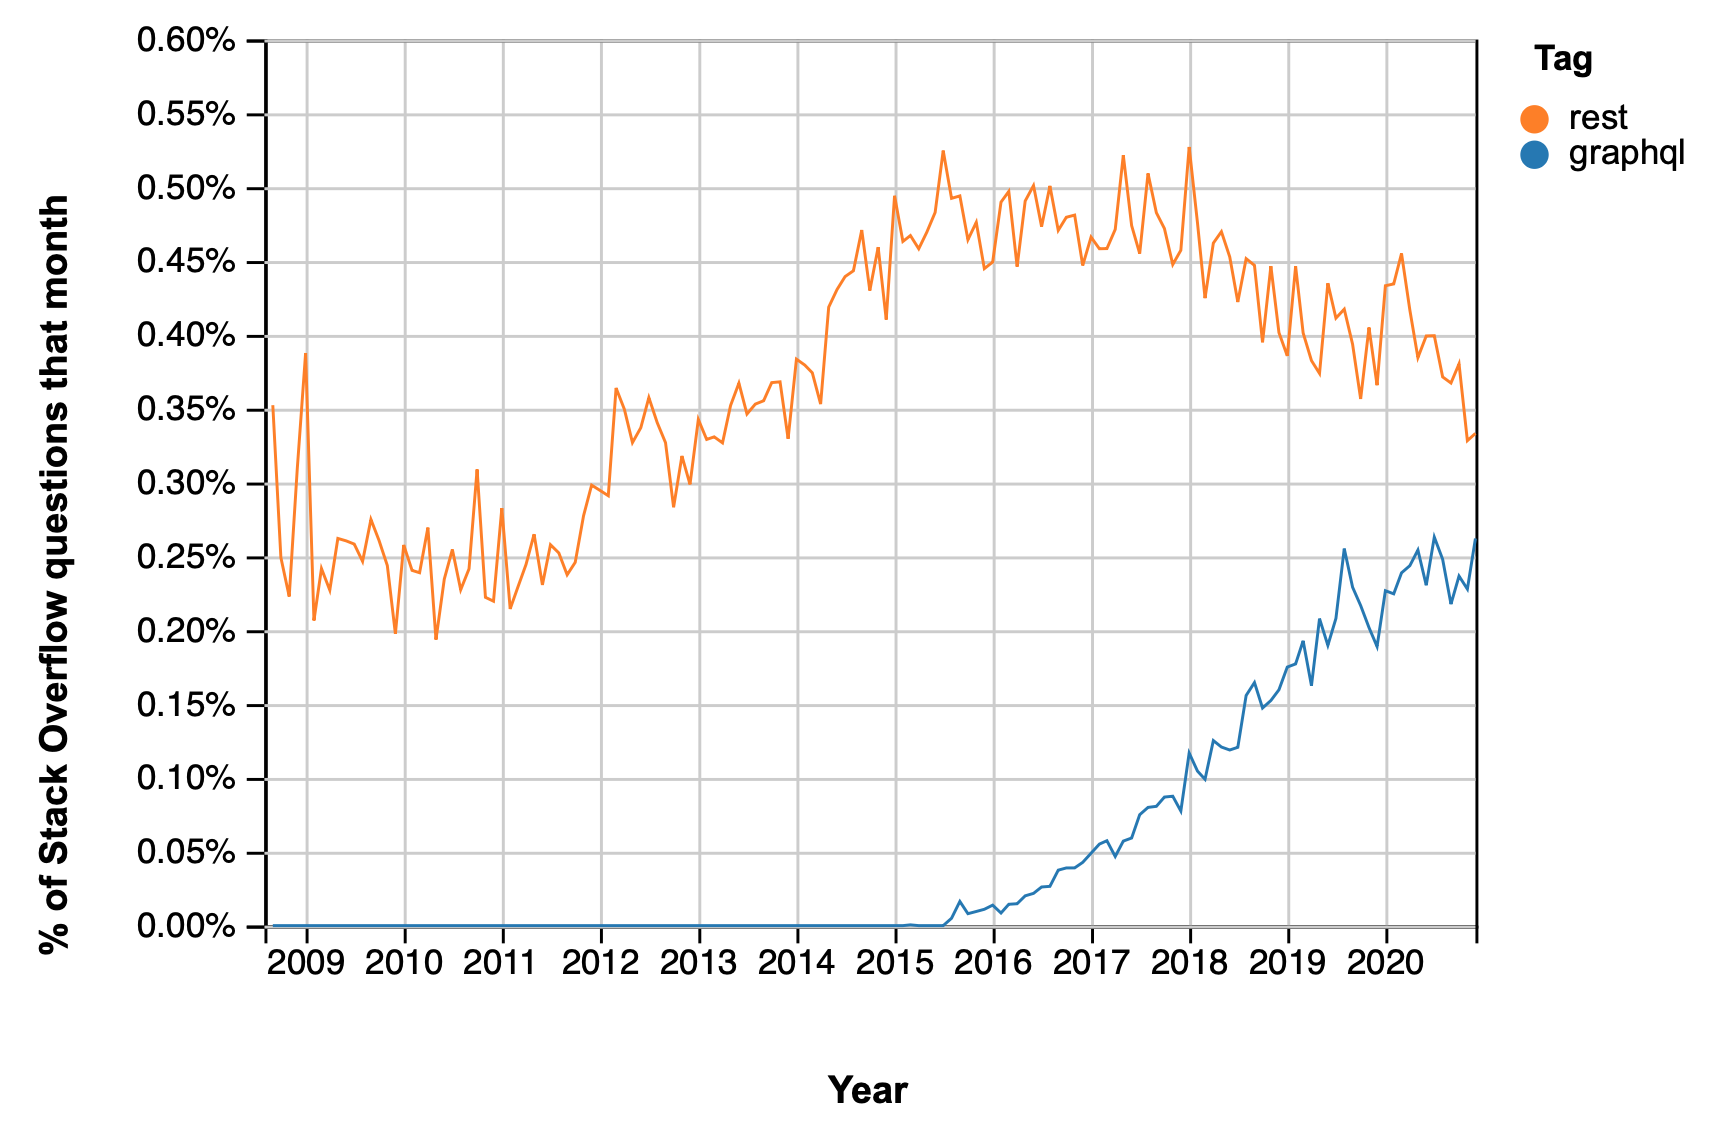
\includegraphics[width=\linewidth]{restvsgraphql}
\copyrightbox[b]{\includegraphics[width=0.9\linewidth]{apis}}%
           {Quelle: \url{https://nordicapis.com/breaking-down-smartbears-2020-state-of-api-report/}}
\end{figure}
 


Aktuell sind REST basierte Schnittstellen Architekturen mit 82\% eindeutig Standard in der Industrie (Abbildung \ref{fig:apis}). Jedoch
deuten die Vorteile bei der technischen Umsetzung, die erfolgreiche Migration größerer Unternehmen zur Verwendung von GraphQL\footnote{https://landscape.graphql.org} und nicht zuletzt die steigende Verwendung bei den Entwicklern (Abbildung \ref{fig:restvsgraphql}) auf eine steigende Bedeutung für die Wirtschaft hin. 

\begin{figure}[H]
\caption{}
\label{fig:restvsgraphql}
\centering
%\setcaptioncitation{\textit{}}
%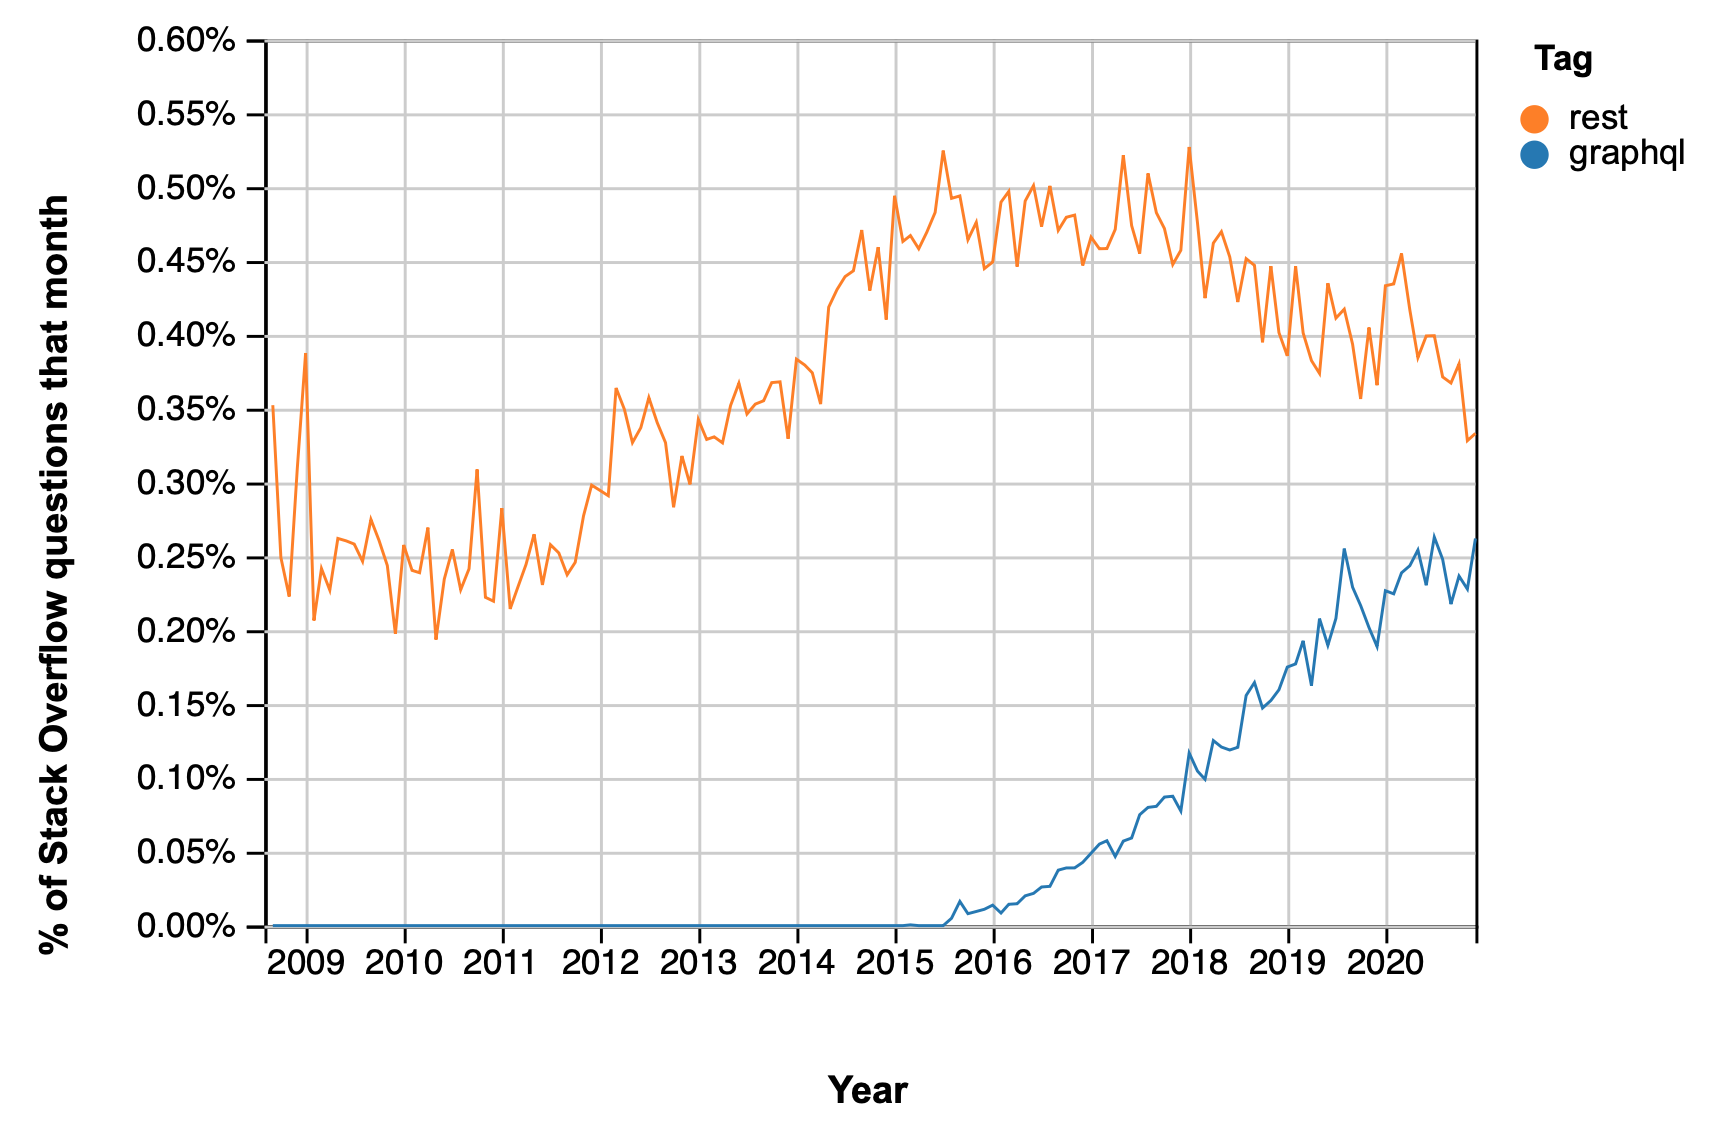
\includegraphics[width=\linewidth]{restvsgraphql}
\copyrightbox[b]{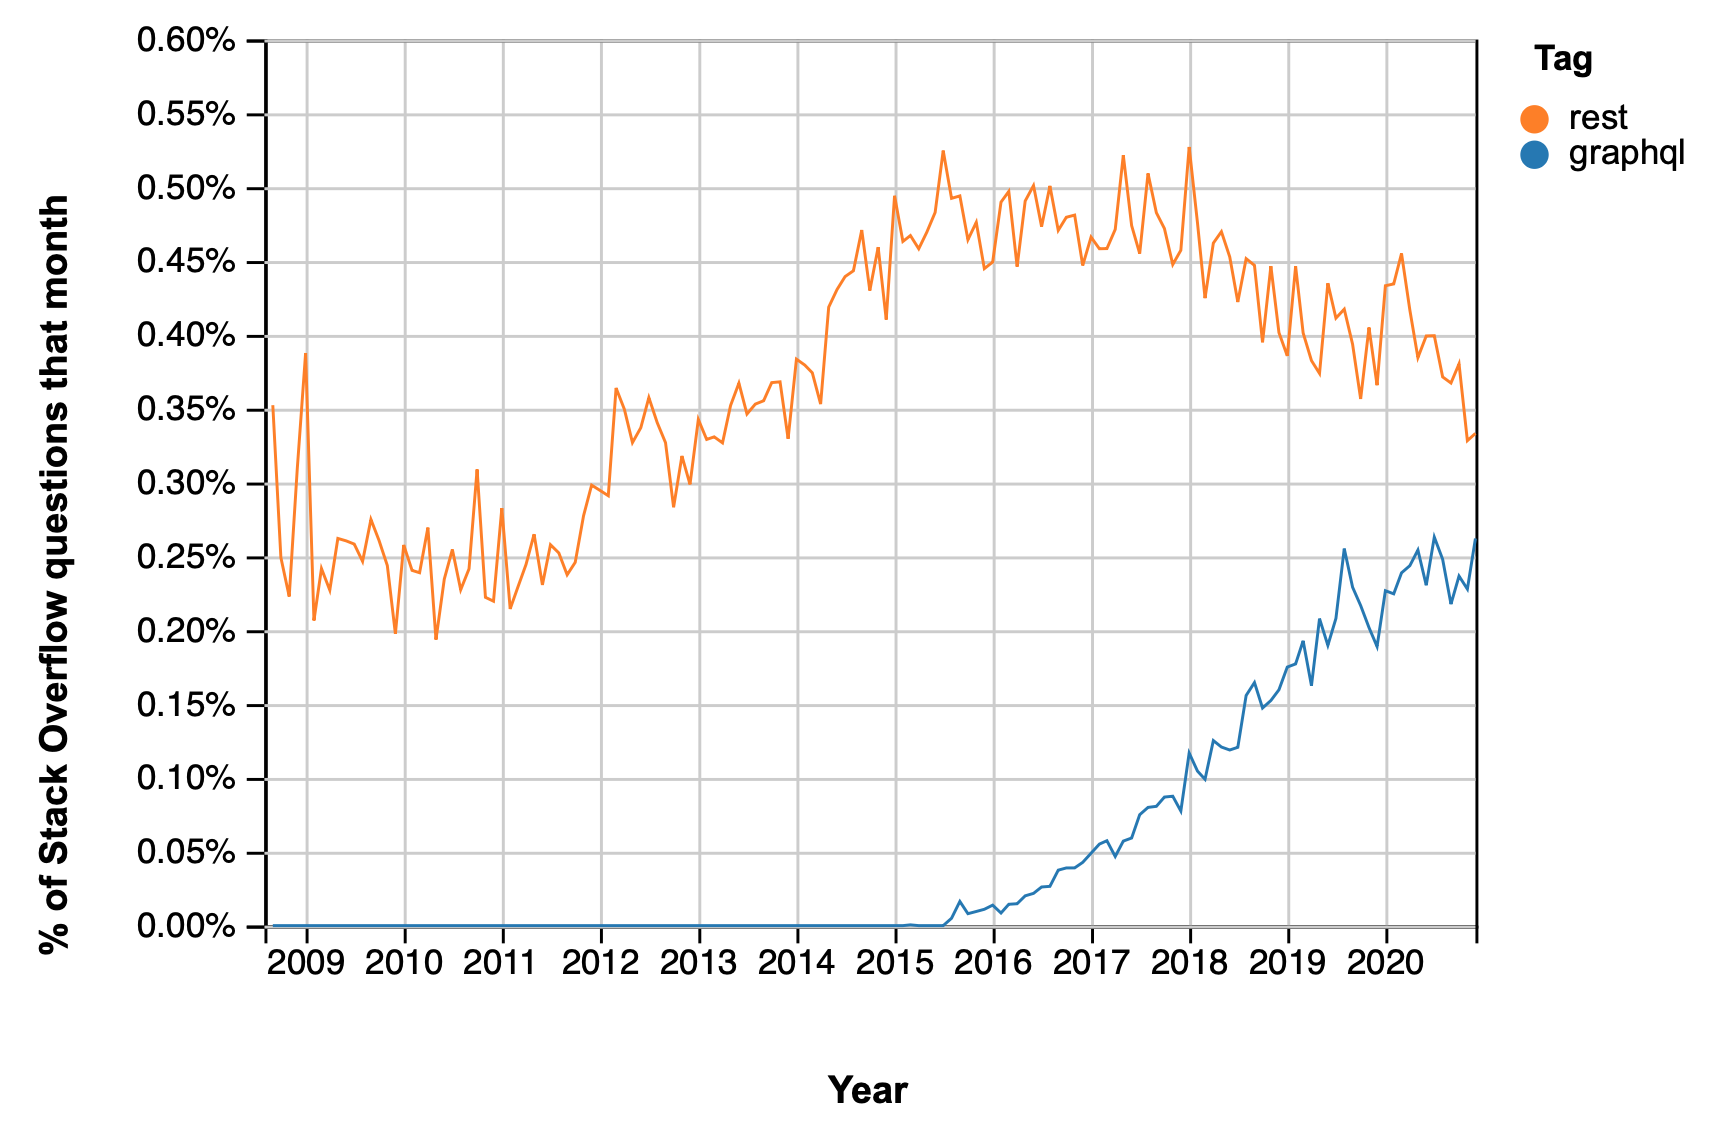
\includegraphics[width=0.9\linewidth]{restvsgraphql}}%
           {Quelle: \url{https://insights.stackoverflow.com/trends?tags=graphql\%2Crest}}
\end{figure}
 
\newpage
\section{Ausblick auf weitere Entwicklungen}
Betrachtet man die Entwicklung der letzten Jahre, kann eine steigende Beschäftigung von Entwicklern mit GraphQL und ein Abnehmen von REST (Abbildung \ref{fig:restvsgraphql}) festgestellt werden. Gerade auch in Anbetracht der steigenden Nutzung mobiler Endgeräte und gleichzeitig steigendem Datentransfer ist eine effiziente und performante Datenabfragesprache wichtig. Darüberhinaus werden Schnittstellen immer komplexer. Um diese Komplexität zu handhaben erscheint GraphQL aufgrund der oben beschriebenen Vorteile attraktiv.


%- Wird etablierte Schnittstellen Architekturen wie REST nicht ersetzen, aber ergänzen/eine alternative darstellen.
%Der Nutzen von GraphQL ist nicht zu bestreiten und es wird daher davon ausgegangen, dass GraphQL 
\end{document}
